\section{Sacred Science 108: The Subtle State}

The Self or Atman, manifests itself as a soul (jivatman) in the living form of the individual human being. It is covered in a series of successive sheaths, or koshas, representing phases of its manifestation.

I am associating the koshas with names of bodies, even thought, apart from the physical or gross body, are not really bodies. Moreover, the names are for convenience and are not tied to any particular school or organization.

Note that one sheath is associated with the spirit or pneuma, and one with the body or soma. There are three associated with the soul or psyche.

\begin{enumerate}
\item \textbf{Anandamayakosha or causal body}: This is the set of all the possibilities of manifestation that Atman contains in itself. It is unconditioned and formless. In relation to the formal manifestation, it is the causal form through which the human being will be manifested and actualized. 
\item \textbf{Mananayakosha or Mental Body}: This sheath is formed by the intelligible Light of universal Knowledge. It consists in joining the superior intellect (Buddhi) to the tanmatras. 
\item \textbf{Manomayakosha or Astral Body}: This includes the mind (manas) and all its activities. 
\item \textbf{Pranamayakosha or etheric body}: This includes the vital breath (prana) and is modalities (vayus). It also includes the faculties of sensation (Buddhindriyas) and of action (karmendriyas). 
\item \textbf{Annamayakosha or gross body}: This is the physical body. It assimilates food to keep the body operational. 
\end{enumerate}

\paragraph{Laws}
At each level, the human being is subjected to increasingly strict laws.

\begin{itemize}
\item \textbf{Causal body}. Since this is unconditioned, it is liberated from all laws and conditions. 
\item \textbf{Mental body}. It is subject to all the laws of thought including logical and mathematical laws. 
\item \textbf{Astral body}. The human being is subject to psychological laws. 
\item \textbf{Etheric body}. The human being is subject to all the biological laws of the system. 
\item \textbf{Gross body}. The physical body is subject to physical and chemical laws. 
\end{itemize}

\paragraph{Subtle State}

Since we already described the gross state in Sacred Science 107: The Heart of the Matter, and will deal with the unconditioned state at a later time, this section will deal with the subtle state.

This requires a more refined description of the three sheaths. There are two factors that need to be considered:

\begin{wrapfigure}{rt}{.35\textwidth}
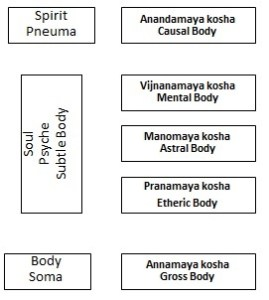
\includegraphics[scale=.5]{a20221113SacredScience108TheSubtleState-img001.jpg}
\caption{The Koshas/Sheaths}
\end{wrapfigure}

\begin{itemize}
\item Like all manifestation, the sheaths are subject to the gunas. Therefore, each sheath has a negative part, a positive part, and a neutralized correlate. 
\item The sheaths are not entirely independent because of the unity of the being. Therefore, the divisions are not sharp, so they blend into each other. These are represented by sectors within the center. 
\end{itemize}
Instead of sheaths, we can regard them as centers within the being. These are the intellectual, emotional, and motor centers, corresponding to the second, third, and fourth sheath respectively.

Note that each center is divided into a positive and negative part (above and below the line).

Because of the interaction of the centers, thoughts, feelings, and actions are seldom pure. Everything is mixed and even entangled. For example, we may not think honestly because our emotions cloud our judgment. Or false intellectual ideas can affect the emotions, causing pleasant emotions from bad ideas.

\paragraph{Intellectual Center}
This center is the focus of discursive thought. It analyzes, calculates, and so on. There is the ability to understand mathematics and logic. The gnomic will, which deliberates alternative courses of action, is also part of this center.

Creative ideas arise from the positive part of the intellectual center, while criticisms come from the negative part. When they are in balance, the creative idea will improve from a critique. But often the negative part will thwart the idea. Irrational and illogical thoughts can also arise from the negative part.

\begin{wrapfigure}{rt}{.35\textwidth}
 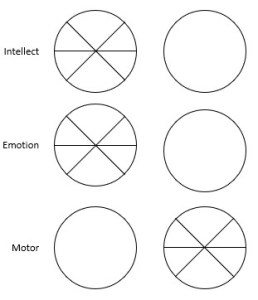
\includegraphics[scale=.5]{a20221113SacredScience108TheSubtleState-img002.jpg} 
 \caption{Centers of Subtle Body}
\end{wrapfigure}

Mechanical thoughts come from the motor sector of the intellectual center. They arise spontaneously. People will just repeat the same comment, often absorbed through propaganda, whether pertinent or not. It is impossible to have an intelligent conversation with someone who thinks mechanically.

The emotional sector will distort thoughts. A strong emotion will usually lead to thinking that justifies the emotional reaction, without any basis in fact.

If one succeeds in neutralizing or reconciling the thinking center, the higher thinking center can arise. That is represented by the circle without a positive and negative part, and without sectors.

\paragraph{Emotional Center}

The is the center of feelings, refined sensations, passions. The stream of consciousness of thoughts and images arise here. If the negative part of this center is in harmony, it completes the positive part. For example, positive emotions are associated with agreeable things and negative emotions with the disagreeable.

But too often, negative emotions like anxiety, depression, anger, fear, and so on come to dominate. This distorts the entire life of the human being. This is verified end by secular standards. That is why esoteric training emphasizes the emotions so much. Again, there is a higher emotional center that can arise by reconciling the positive and negative parts.


\paragraph{Motor Center}
The senses comprise the positive part of the motor center and the negative part includes the faculties of action. Being mostly subconscious, the motor center is the best functioning center in most human beings. It is important to keep it as healthy as possible.

The sexual center is represented by the undivided circle. However, the purification of the sexual center is a discussion for another time.

\flrightit{Posted on 2022-11-13 by Cologero}

\begin{center}* * *\end{center}

\begin{footnotesize}\begin{sffamily}

\hfill

\texttt{Logres on 2022-11-19 at 18:55 said: }

This elucidates with precision and insight. In particular, the statement that balancing the negative and positive parts of a center leads to the arising of the pure center, was creatively well put, and sheds more and more light. This connects practical experience of purification with the somewhat more abstract and mysterious teachings in Mouravieff's work, about higher centers, and ties it into the Gunas. I'm constantly amazed at the connections you make, and find myself more than several steps behind. God speed all your endeavors.


\hfill

\texttt{Dimitri on 2022-11-20 at 18:31 said: }

Both yourself and Cologero have done a great service to us all, Logres. I truly appreciate both of your insights, your posts are always a pleasure to read. This site is full of so many gems, there's no other site out there like Gornahoor.

\end{sffamily}\end{footnotesize}